\documentclass[12pt]{article}
\usepackage{amsmath}
\usepackage{multirow}
\usepackage{enumerate}
\usepackage{graphicx}
\usepackage{changepage}
\usepackage[all]{xy}
\usepackage{tikz}
\usetikzlibrary{shapes}
\usepackage{color}

\setlength{\voffset}{-3cm}
%\setlength{\hoffset}{-2cm}
%\setlength{\parindent}{0cm}
\setlength{\textheight}{26cm}
%\setlength{\textwidth}{14cm}
\newcommand{\tcr}{\textcolor{red}}

\begin{document}


\begin{center}
{\bf\Huge TEMPLATE EXAM\\[0.5cm]}
\quad\\[1cm]
\begin{adjustwidth}{-1cm}{0cm}
\begin{tabular}{l@{\qquad}l}
MODULE CODE: MA4413&SEMESTER: Autumn 2015\\[1cm]
MODULE TITLE: Statistics for Computing& DURATION OF EXAM: 2.5 hours\\[1cm]
LECTURER: Dr.~Kevin Burke& GRADING SCHEME: 100 marks \\
& \hspace{3cm} (60\% of module)\\[2cm]
%EXTERNAL EXAMINER:&\\
%Prof. Brendan Murphy&\\[1cm]
\end{tabular}
\end{adjustwidth}
{\bf INSTRUCTIONS TO CANDIDATE}
\end{center}
\begin{small}
\begin{itemize}\itemsep0.3cm
\item {\bf Attempt four} of the six questions (each one carries 25 marks).
\item {All work must be shown \emph{clearly and logically} using appropriate symbols and probability notation. Failure to do so will \emph{lose marks}.}
\item {Write down the formula you intend to use at each stage \emph{before} filling it in with numbers.}
\item Formula sheets are provided at the back of this exam paper.
\item Statistical tables are available from the invigilators.
\end{itemize}
\end{small}
\newpage

\noindent{\bf Note}: Exam questions are based on the examples and questions from lectures and tutorials. You have the solutions to all questions on this course. Below is the layout of the exam in terms of the lectures (you can find the corresponding tutorial questions yourself). Lec 5 (counting techniques) and Lec 17 (chi-squared test) are not examinable this year.

\section*{Question 1}
\begin{enumerate}[a)]
\item Probability basics (Lec 3 and 4)
\item Boxplots / numerical summaries (Lec 2)
\item Hypothesis test / confidence interval for one parameter, i.e., $\mu$ or $p$ (Lec 13, 14, 15 and 16)
\end{enumerate}

\section*{Question 2}
\begin{enumerate}[a)]
\item Histogram / numerical summaries (Lec 1 and 2)
\item Statistic and parameter / numerical summaries (Lec 1 and Lec 2)
\item Probability (law of total probability) (Lec 3 and 4)
\end{enumerate}

\section*{Question 3}
\begin{enumerate}[a)]
\item Numerical summaries (Lec 2)
\item Confidence interval based on large sample(s) (Lec 13)
\item Hypothesis test based on large sample(s) (Lec 15 and 16)
\end{enumerate}

\section*{Question 4}
\begin{enumerate}[a)]
\item Random variables (Lec 6)
\item Binomial (Lec 7)
\item Poisson and Exponential (Lec 8 and 9) but \emph{not} queueing theory here
\end{enumerate}


\section*{Question 5}
\begin{enumerate}[a)]
\item Huffman coding and entropy (Lec 18)
\item Normal distribution (Lec 10, 11 and 12)
\end{enumerate}


\section*{Question 6}
\begin{enumerate}[a)]
\item Confidence interval or hypothesis test for difference between two means (i.e., $\mu_1-\mu_2$) based on small samples (Lec 14 and 16)
\item Queueing theory (Lec 8 and 9)
\end{enumerate}




\newpage














\section*{Useful Formulae: Page 1\\[0.3cm]}
{\bf Histogram:}\\[-0.8cm]
\begin{align*}
\bullet\quad \text{class width} = \frac{\max(x) - \min(x)}{\text{number of classes}}\\
\end{align*}
{\bf Numerical Summaries:}\\[-0.8cm]
\begin{align*}
\bullet\quad \bar x &= \frac{\sum\,x_i}{n}\\[0.6cm]
\bullet\quad s^2 &= \frac{\sum\,x_i^2 - n\,\bar x^2}{n-1}\\[0.6cm]
\bullet\quad \text{Position of } Q_k:& \quad \frac{n+1}{4}\times k \\[0.6cm]
\bullet\quad IQR &= Q_3 - Q_1 \\[0.6cm]
\bullet\quad LF &= Q_1 - 1.5 \times IQR \\[0.6cm]
\bullet\quad UF &= Q_3 + 1.5 \times IQR\\
\end{align*}
{\bf Probability:}\\[-0.8cm]
\begin{align*}
\bullet\quad \Pr(A^c) &= 1 - \Pr(A) \\[1cm]
\bullet\quad \Pr(A \cup B) &= \Pr(A) + \Pr(B) - \Pr(A \cap B)\\[0.6cm]
\bullet\quad \Pr(E_1 \cup E_2 \cup \cdots \cup E_k) &= \Pr(E_1) + \Pr(E_2) + \cdots + \Pr(E_k) \text{\quad{\footnotesize(if mutually exclusive)}}\\[1cm]
\bullet\quad \Pr(A \cap B) &= \Pr(A) \, \Pr(B \, | \, A) = \Pr(B) \, \Pr(A \, | \, B) \\[0.6cm]
\bullet\quad \Pr(E_1 \cap E_2 \cap \cdots \cap E_k) &= \Pr(E_1) \, \Pr(E_2) \, \cdots \, \Pr(E_k) \text{\quad{\footnotesize(if independent)}}\\[1cm]
\bullet\quad \Pr(A\,|\,B) &= \frac{\Pr(A \cap B)}{\Pr(B)} = \frac{\Pr(A) \,\Pr(B\,|\,A)}{\Pr(B)}\\[1cm]
\bullet\quad \Pr(B) = \Pr(B \cap E_1) &+ \Pr(B \cap E_2) + \cdots + \Pr(B \cap E_k) \\[0.2cm]
= \Pr(E_1) \, \Pr(B\,|\,&E_1) + \Pr(E_2) \, \Pr(B\,|\,E_2) + \cdots + \Pr(E_k) \, \Pr(B\,|\,E_k)\\[0.1cm]
\text{{\footnotesize(if $E_1,\ldots, E_k$}} & \,\, \text{{\footnotesize are mutually exclusive \& exhaustive)}}
\end{align*}

\newpage

\section*{Useful Formulae: Page 2\\[0.3cm]}
{\bf Counting Techniques:}\\[-0.8cm]
\begin{align*}
\bullet\quad n\,! &= n\times(n-1)\times(n-2)\times\cdots\times3\times2\times 1\\[0.6cm]
\bullet\quad \binom{n}{k} &= \frac{n\,!}{k\,! \,(n-k)\,!}\\
\end{align*}
{\bf Random Variables:}\\[-0.8cm]
\begin{align*}
\bullet\quad E(X) &= \sum x_i \,\, p(x_i)\\[0.6cm]
\bullet\quad E(X^2) &= \sum x_i^2 \,\, p(x_i)\\[0.6cm]
\bullet\quad Var(X) &= E(X^2) - [E(X)]^2\\[0.6cm]
\bullet\quad Sd(X) &= \sqrt{Var(X)}\\
\end{align*}
{\bf Distributions:}\\[-0.0cm]
\begin{adjustwidth}{-2.1cm}{0cm}
\begin{tabular}{|c@{\quad}|c@{\quad}|c@{\quad}|}
\hline
&&\\[-0.3cm]
$\bullet\quad X \sim \text{Binomial}(n,p)$ & $\bullet\quad X \sim \text{Poisson}(\lambda)$ & $\bullet\quad T \sim \text{Exponential}(\lambda)$ \\[0.6cm]
${\displaystyle\bullet\quad \Pr(X=x) = \binom{n}{x}\,p^x\,(1-p)^{n-x}}$ & ${\displaystyle\bullet\quad \Pr(X=x) = \frac{\lambda^x}{x\,!}\,\,e^{-\lambda}}$ & $\bullet\quad \Pr(T>t) = e^{-\lambda\,t}$ \\[0.8cm]
$\bullet\quad x \in \{0,1,2,\ldots,n\}$ & $\bullet\quad x \in \{0,1,2,\ldots,\infty\}$ & $\bullet\quad t \in [0,\,\infty)$ \\[0.8cm]
$\bullet\quad E(X) = n\,p$ & $\bullet\quad E(X) = \lambda$ & ${\displaystyle\bullet\quad E(T) = \frac{1}{\lambda}}$ \\[0.8cm]
$\bullet\quad Var(X) = n\,p\,(1-p)$ & $\bullet\quad Var(X) = \lambda$ & ${\displaystyle\bullet\quad Var(T) = \frac{1}{\lambda^2}}$ \\[0.4cm]
\hline
\multicolumn{3}{c}{}\\
\multicolumn{3}{c}{{\bf Note: the normal distribution is shown on the next page}}
\end{tabular}
\end{adjustwidth}




\newpage

\section*{Useful Formulae: Page 3\\[0.3cm]}
{\bf Queueing Theory:}\\[-0.8cm]
\begin{align*}
\bullet\quad E(N) &= \lambda_a\,E(T)\\[0.6cm]
\bullet\quad \rho &= \frac{\lambda_a}{\lambda_s}\\[0.6cm]
\xymatrixcolsep{0.5cm}
\bullet\quad M/M/1 \text{ System:} \quad & \xymatrix{\lambda_a \ar@{->}[r] & \hspace{-0.1cm}
{\begin{tabular}{@{}c|@{}c|@{}c|@{}c|@{}c|@{}c}
\cline{1-5}
&&&& &
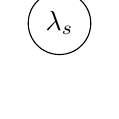
\begin{tikzpicture}[baseline=(char.base)]
\node(char)[draw,shape=circle]{$\lambda_s$};
\end{tikzpicture}\\
\cline{1-5}
\end{tabular}} \hspace{-0.3cm}\ar@{->}[r] &  \lambda_a} \\[0.6cm]
&\Rightarrow \,\, T \sim \text{Exponential}(\lambda_s-\lambda_a)\\[0.1cm]
{\footnotesize(\text{where $T$}} & {\footnotesize\text{ is the total time in the system)}}\\
\end{align*}

{\bf Normal Distribution:}\\[-0.6cm]
\begin{align*}
\bullet\quad X \sim \text{Normal}&(\mu,\sigma) \\[0.4cm]
\bullet\quad E(X) &= \mu \\[0.4cm]
\bullet\quad Var(X) &= \sigma^2 \\[0.4cm]
\bullet\quad (1-\alpha)100\% \text{ of the Normal}(\mu,\sigma) & \text{ distribution lies in } \mu \pm z_{\,\alpha/2}\,\,\sigma \\[0.4cm]
\bullet\quad \Pr(X > x) &= \Pr\left(Z> \frac{x-\mu}{\sigma}\right)\\[1cm]
\bullet\quad \Pr(Z < -z) &= \Pr(Z > z) \\[0.6cm]
\bullet\quad \Pr(Z > -z) &= \Pr(Z < z) = 1 -\Pr(Z>z) \\[1cm]
\bullet\quad \text{If} \,\,  X_1 \sim \text{Normal}(\mu_1,\sigma_1) \,\,  & \text{ and } \,\, X_2 \sim \text{Normal}(\mu_2,\sigma_2) \\[0.4cm]
\Rightarrow \quad  \text{ Sum: } \quad  X_1 + X_2 &\sim \text{Normal}\left(\mu_1+\mu_2,\,\sqrt{\sigma_1^2+\sigma_2^2}\,\right) \\[0.4cm]
\Rightarrow \quad  \text{ Difference: } \quad   X_1 - X_2 &\sim \text{Normal}\left(\mu_1-\mu_2,\,\sqrt{\sigma_1^2+\sigma_2^2}\,\right) \\[1cm]
\bullet\quad \text{For} \,\,  X_1,\ldots,X_n \sim \text{any distribution} & \text{ with } \mu = E(X) \text{ and } \sigma = Sd(X) = \sqrt{Var(X)}\\[0.4cm]
\Rightarrow \quad  \text{ Sample mean: } \quad  \,\overline{\!X} &\sim \text{Normal}\left(\mu,\,\frac{\sigma}{\sqrt{n}}\,\right) \quad \text{ if } n > 30
\end{align*}

\newpage


\section*{Useful Formulae: Page 4\\[0.3cm]}
{\bf Statistics and Standard Errors:}\\[0.1cm]
\begin{adjustwidth}{-2cm}{0cm}
\begin{tabular}{|c|c|c|c|c|}
\hline
&&&&\\[-0.1cm]
Parameter & Statistic & Standard Error & Samples & Details \\[0.3cm]
\hline
&&&&\\[-0.1cm]
$\mu$ & $\bar x$ & ${\displaystyle\frac{s}{\sqrt{n}}}$  & large / small & $\nu = n - 1$ \\[0.5cm]
\hline
&&&&\\[-0.1cm]
$p$ & $\hat p$ & \multirow{2}{*}{${\displaystyle\sqrt{\frac{\hat p\,(1-\hat p)}{n}}}$} & large & confidence \\[-0.1cm]
&&&&interval\\[0.3cm]
\cline{3-5}
&&&&\\[-0.1cm]
&  & \multirow{2}{*}{${\displaystyle\sqrt{\frac{p_0\,(1-p_0)}{n}}}$} & large & hypothesis \\[-0.1cm]
&&&&test\\[0.3cm]
\hline
&&&&\\[-0.1cm]
$\mu_1-\mu_2$ & $\bar x_1 - \bar x_2$ & \multirow{3}{*}{${\displaystyle\sqrt{\frac{s_1^2}{n_1}+\frac{s_2^2}{n_2}}}$} & large / small & ${\displaystyle \nu = \frac{(a+b)^2}{\frac{a^2}{n_1-1}+\frac{b^2}{n_2-1}}}$ \\[0.8cm]
&&&& ${\displaystyle a=\frac{s_1^2}{n_1}, \,\,\, b=\frac{s_2^2}{n_2}}$ \\[0.5cm]
\cline{3-5}
&&&&\\[-0.1cm]
&  & ${\displaystyle\sqrt{\frac{s_p^2}{n_1}+\frac{s_p^2}{n_2}}}$ & small & $\nu = n_1+n_2-2$ \\[0.5cm]
&&&& assuming \\[-0.2cm]
&& where\,\, ${\displaystyle s_p^2 = \frac{(n_1-1)\,s_1^2+(n_2-1)\,s_2^2}{n_1+n_2-2}}$  && $\sigma_1^2 = \sigma_2^2$ \\[0.5cm]
\hline
&&&&\\[-0.1cm]
$p_1-p_2$ & $\hat p_1 - \hat p_2$ & \multirow{2}{*}{${\displaystyle\sqrt{\frac{\hat p_1 \, (1-\hat p_1)}{n_1}+\frac{\hat p_2 \, (1-\hat p_2)}{n_2}}}$} & large & confidence\\[-0.1cm]
&&&&interval\\[0.5cm]
\cline{3-5}
&&&&\\[-0.1cm]
&  & ${\displaystyle\sqrt{\frac{\hat p_c\,(1-\hat p_c)}{n_1}+\frac{\hat p_c\,(1-\hat p_c)}{n_2}}}$ & large & hypothesis\\[-0.4cm]
&&&&test\\[0.2cm]
&&where\,\, ${\displaystyle \hat p_c = \frac{x_1+x_2}{n_1+n_2}}$&&\\[0.5cm]
\hline
\multicolumn{5}{c}{}\\[0.5cm]
\end{tabular}
\end{adjustwidth}
{\bf Confidence Intervals:}\\[-0.5cm]
\begin{align*}
\bullet\quad \text{Large sample:} \qquad \text{statistic } &\pm\,\, z_{\,\alpha/2}\,\times\,\text{standard error} \\[0.6cm]
\bullet\quad \text{Small sample:} \qquad \text{statistic } &\pm\,\, t_{\,\nu,\,\alpha/2}\,\times\,\text{standard error}
\end{align*}

\newpage

\section*{Useful Formulae: Page 5\\[0.3cm]}
{\bf Hypothesis Testing:}\\[-0.5cm]
\begin{align*}
\bullet\quad z &= \frac{\text{statistic}-\text{hypothesised value}}{\text{standard error}} \\[1cm]
\bullet\quad \text{p-value } &= \left\{
\begin{array}{rl}
2 \times \Pr(Z > |z|) & \text{if }  H_a: \, \mu \ne \mu_0\\[0.4cm]
\Pr(Z < z) & \text{if } H_a: \, \mu < \mu_0\\[0.4cm]
\Pr(Z > z) & \text{if } H_a: \, \mu > \mu_0\\
\end{array} \right.\\[1cm]
\bullet\quad F &= \frac{\text{larger variance}}{\text{smaller variance}} = \frac{s_{\text{larger}}^2}{s_{\text{smaller}}^2} \\[0.5cm]
 & \nu_1 = n_{\text{\,top}} - 1,\quad\, \nu_2 = n_{\text{\,bottom}} - 1 \\[1cm]
\bullet\quad \chi^2 &= \sum \frac{(o_i-e_i)^2}{e_i}\\[0.5cm]
\text{Goodness-of-fit: } \qquad &e_i = \text{total} \times p(x_i),\qquad \nu = n_f - 1- k \\[0.6cm]
\text{Independence: } \qquad &e_{ij} = \frac{r_i\,\times\,c_j}{\text{total}},\qquad \nu = (n_r - 1)\,\times\,(n_c - 1)\\[0.3cm]
\end{align*}
{\bf Information Theory:}\\[-0.5cm]
\begin{align*}
\bullet\quad h(x) &= - \log_2[p(x)] \\[0.6cm]
\bullet\quad H(X) &= E[h(X)] = \sum h(x_i)\,p(x_i) \\[1cm]
\bullet\quad l(x_i) &= \text{code-length for character } x_i \\[0.6cm]
\bullet\quad E(L) &= \sum l(x_i)\,p(x_i) \\[1cm]
\bullet\quad e &= \frac{H(X)}{E(L)} \\[1cm]
\bullet\quad &\sum 2^{-l(x_i)}  \le 1
\end{align*}


\end{document}

